\begin{frame}\frametitle{Total and Differential Cross Section}
\begin{table}[h]
  \tiny
  \begin{center}
  %\caption{Relative uncertainties [\%]. $W\gamma$, muon channel.}
   \begin{tabular}{|l|c|}
    \hline
                & $\sigma$ ($P_T^{\gamma}>15$~GeV), fb \\ \hline
    NLO theory  & 9101 \\ \hline
    Data, muon channel & 10949 \pm 91 \pm 1463  \\ \hline
    Data, electron channel & 9146 \pm 185 \pm 2213  \\ \hline
  \end{tabular}
  \end{center}
\end{table}
\begin{figure}[htb]
  \begin{center}
   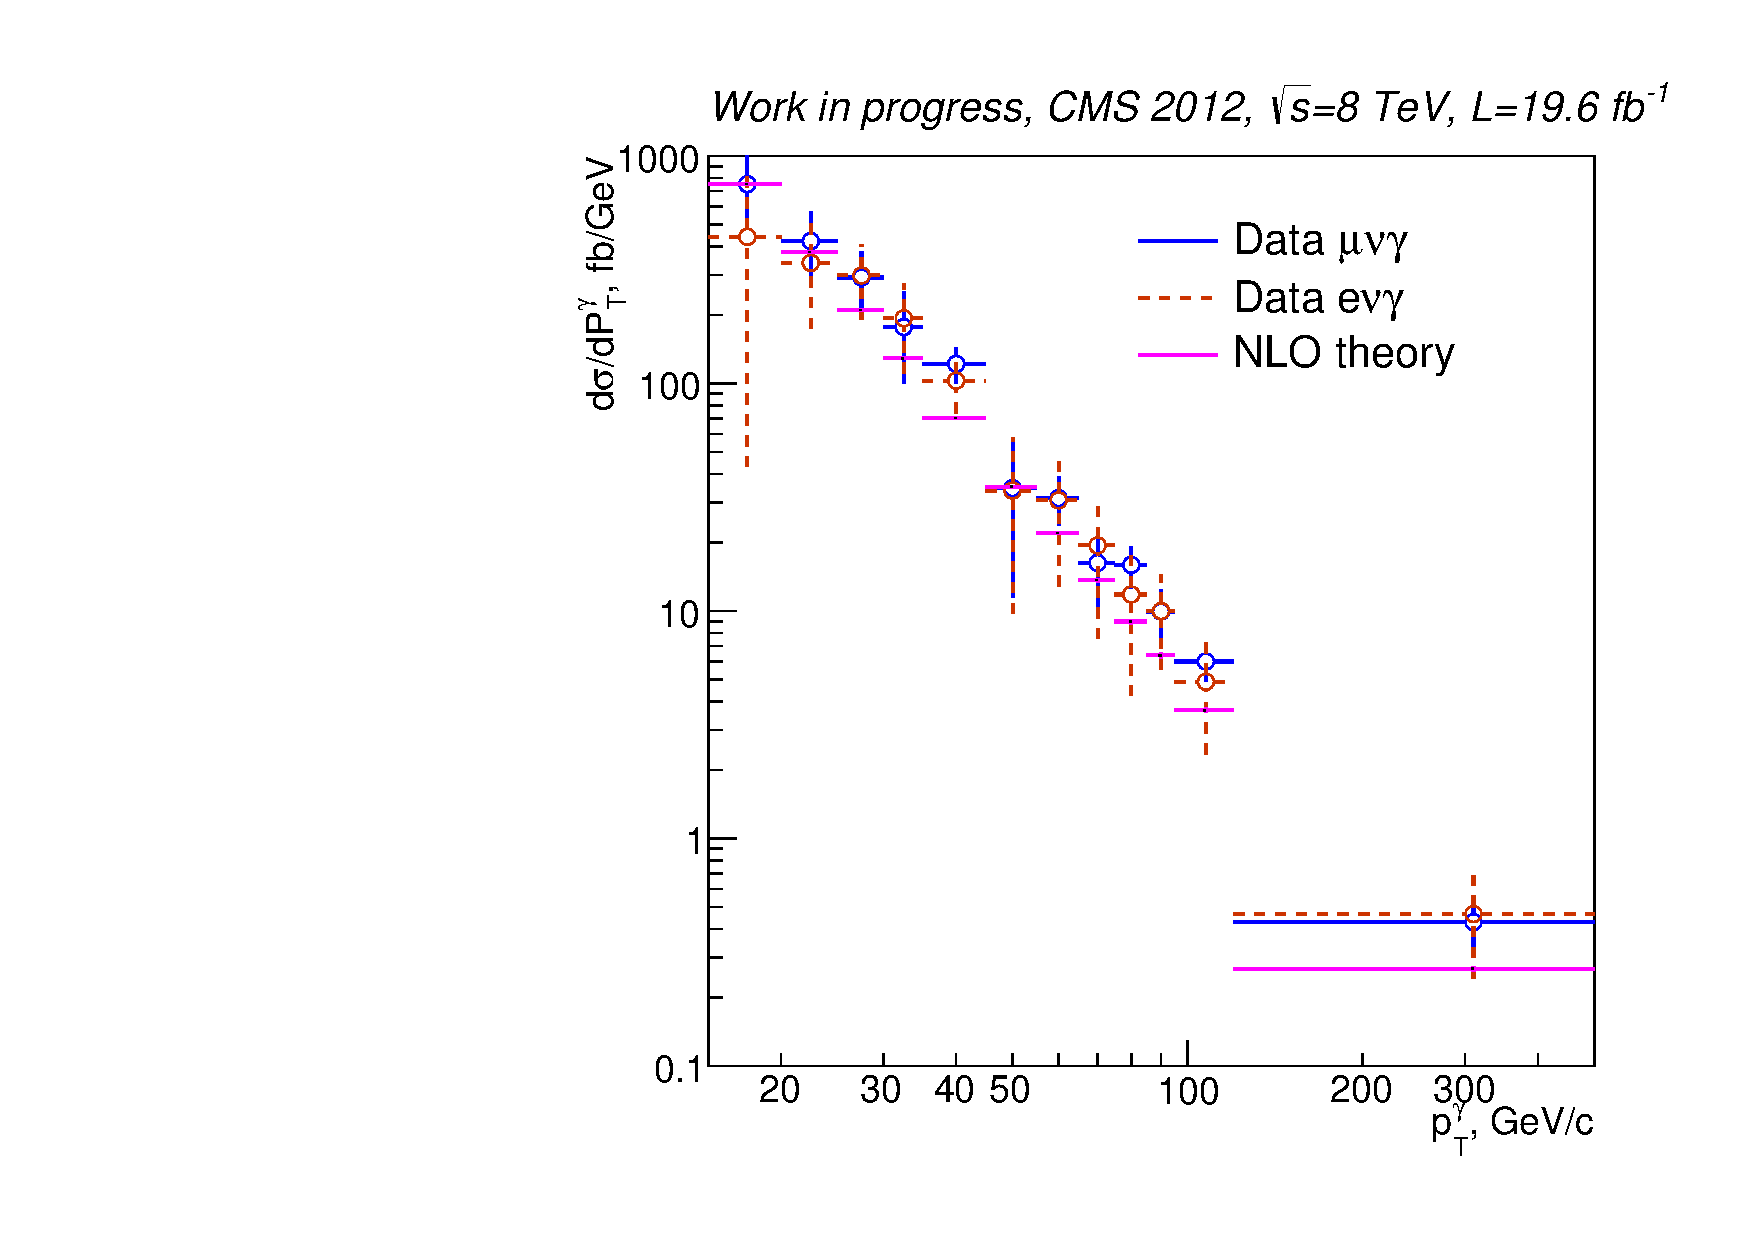
\includegraphics[width=0.49\textwidth]{../figs/figs_v11/ChannelsMERGED_WGamma/CrossSection/compareCSWGamma.pdf}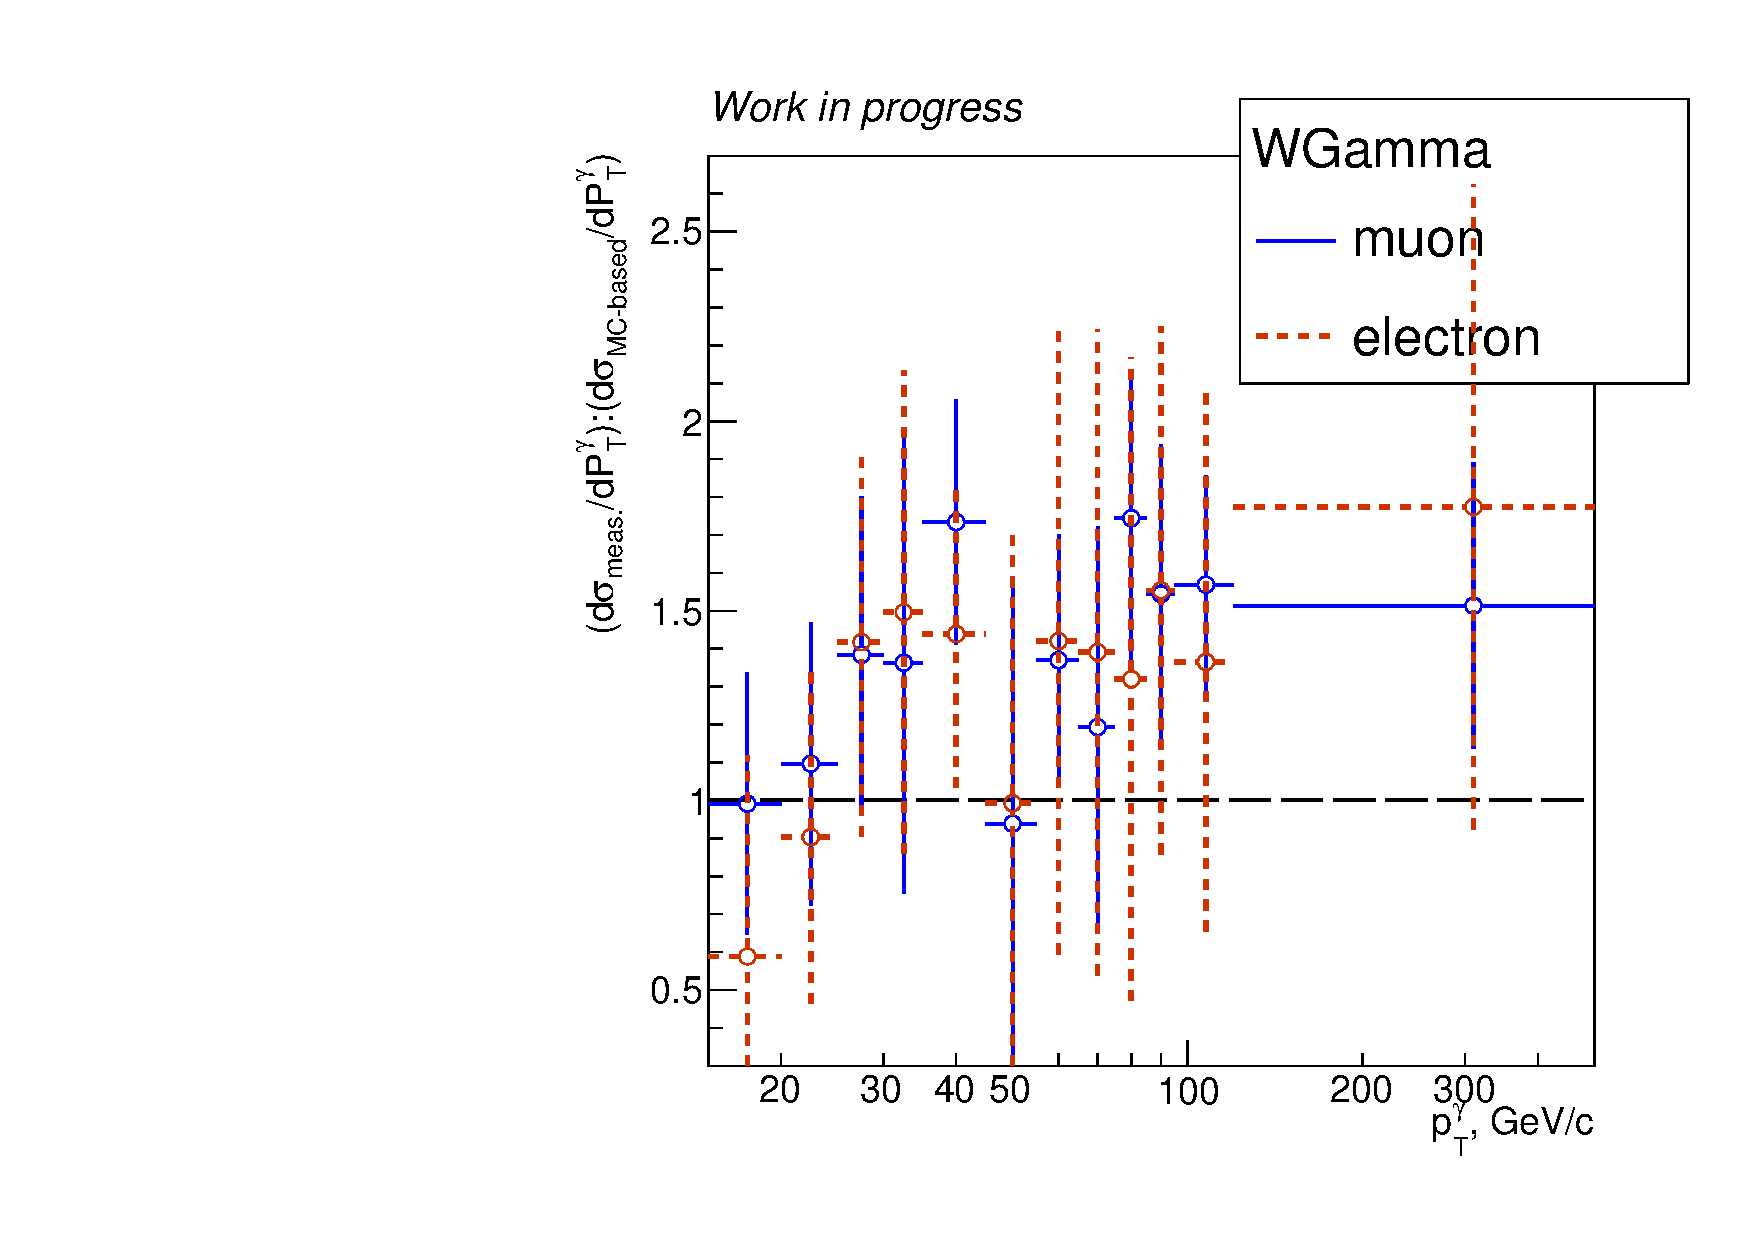
\includegraphics[width=0.49\textwidth]{../figs/figs_v11/ChannelsMERGED_WGamma/CrossSection/compareCSratioTheoryWGamma.pdf}\\
  \end{center}
\end{figure}

\end{frame}%{Differential Cross Section. Plots}

\begin{frame}\frametitle{$Z\gamma$ Check. Differential Cross Section}
\begin{figure}[htb]
  \begin{center}
 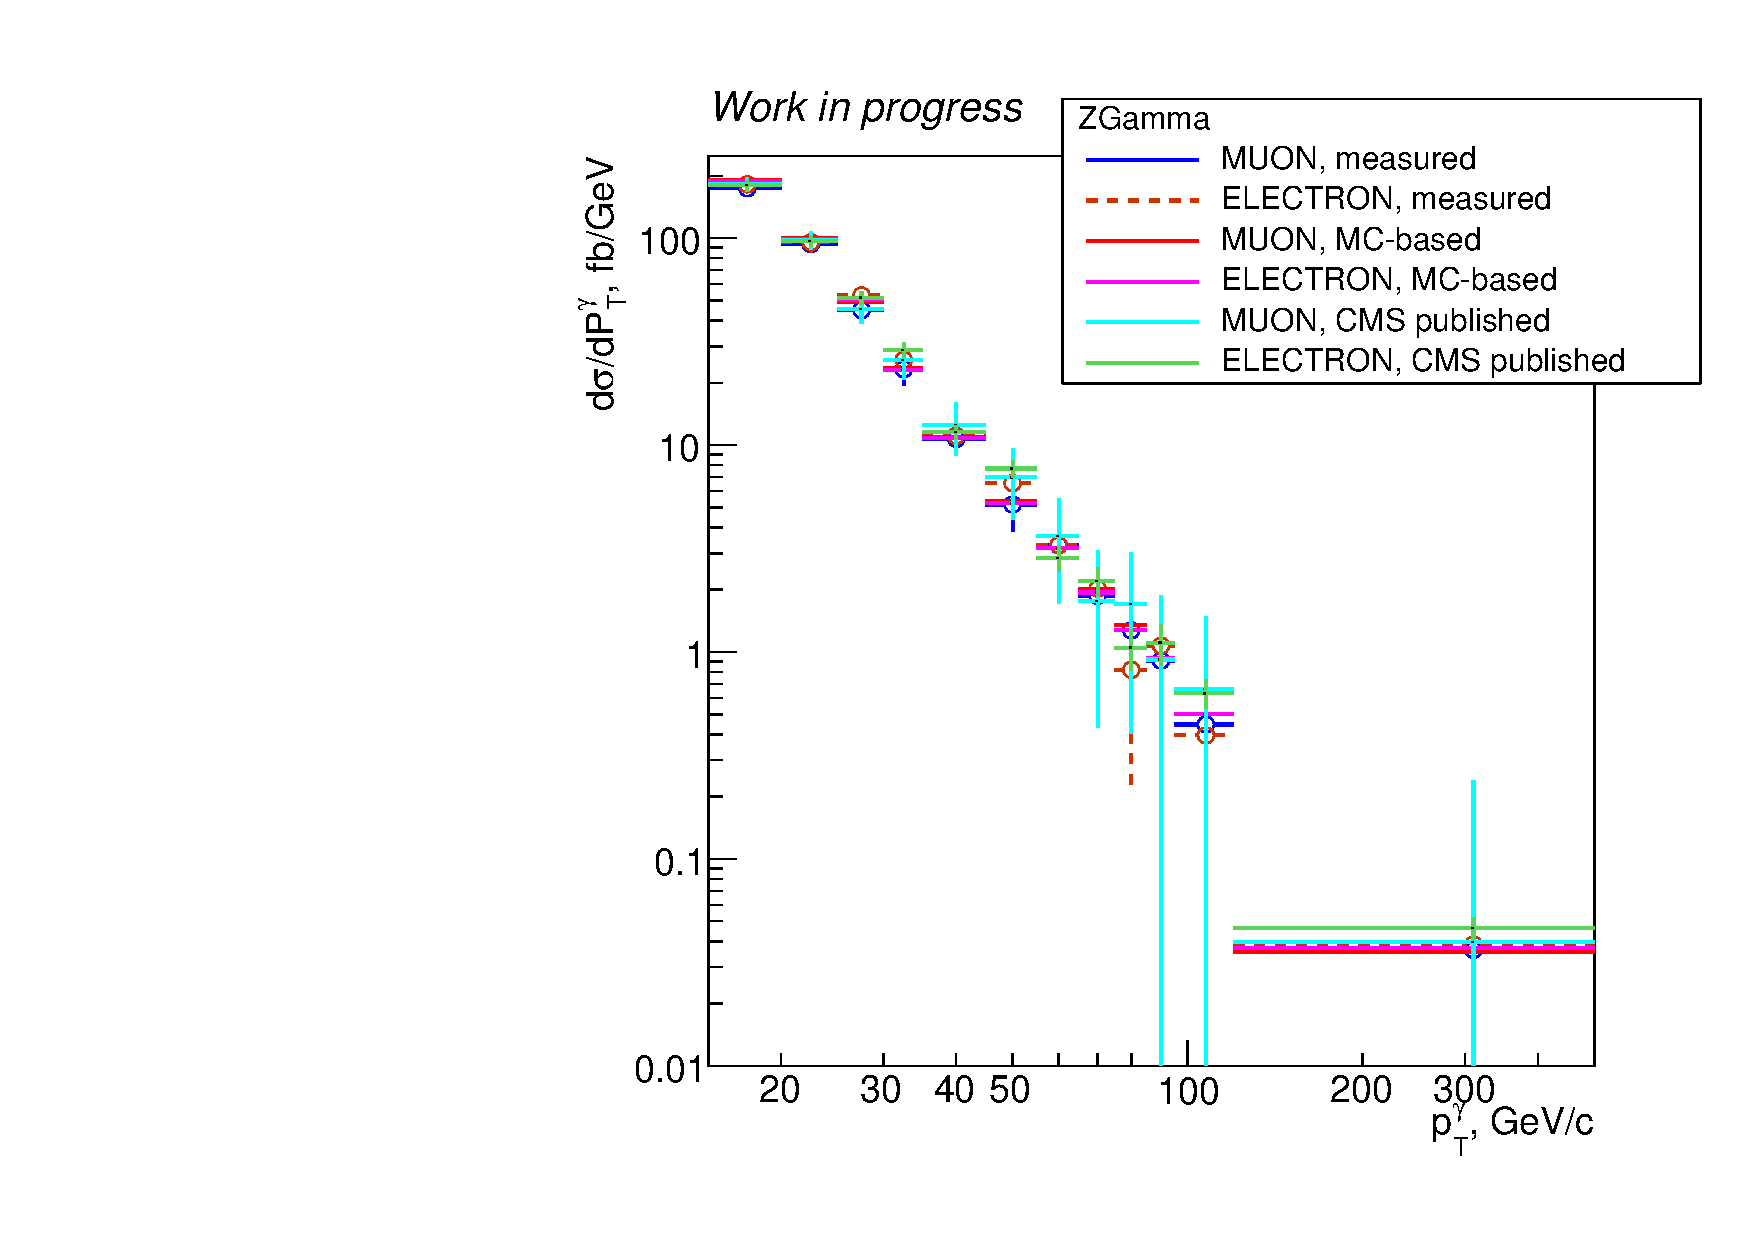
\includegraphics[width=0.49\textwidth]{../figs/figs_v11/ChannelsMERGED_ZGamma/CrossSection/compareCSZGamma.pdf}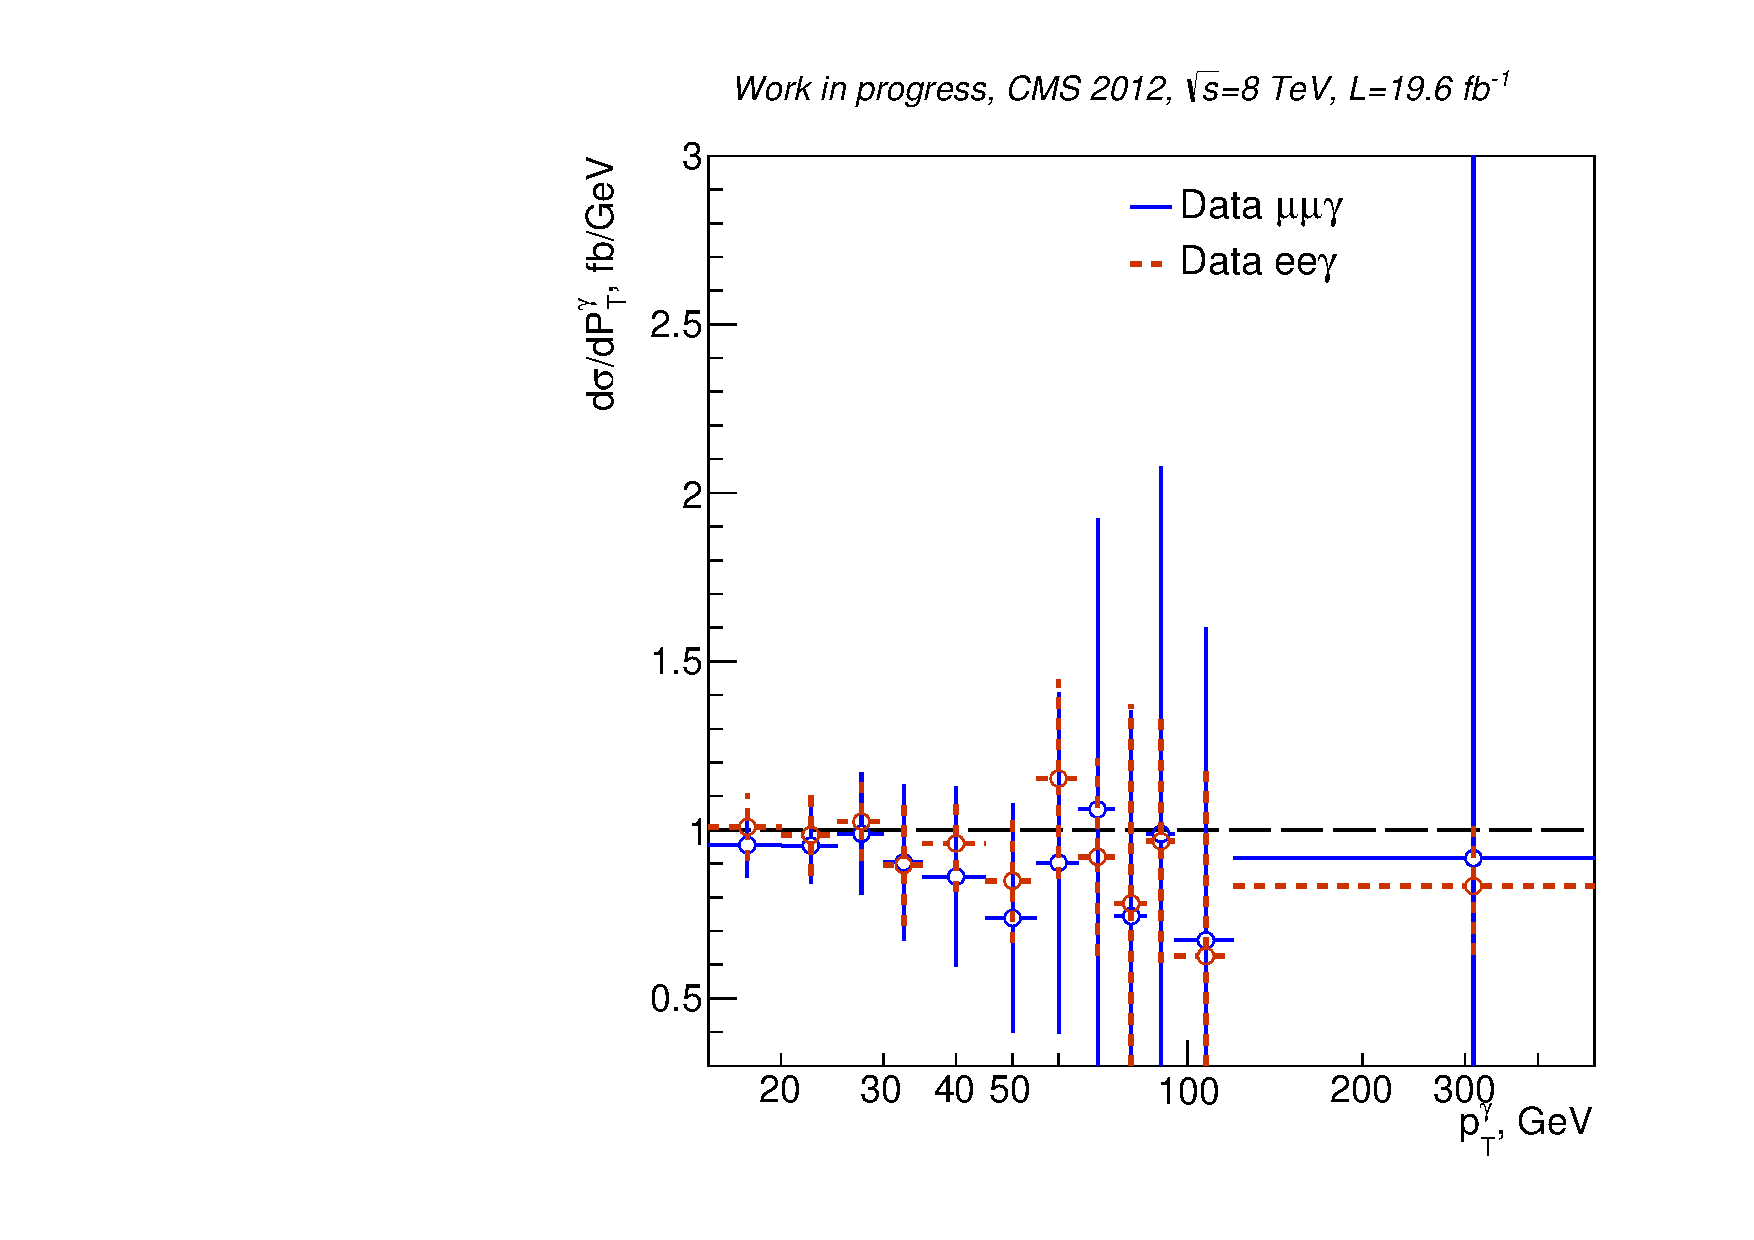
\includegraphics[width=0.49\textwidth]{../figs/figs_v11/ChannelsMERGED_ZGamma/CrossSection/compareCSratioOttoZGamma.pdf}
  \end{center}
\end{figure}
  \tiny
  \begin{itemize}
    \item Cross section of $Z\gamma\rightarrow ll\gamma$ agrees well with the 8 TeV published CMS result and with the theory prediction;
     \item The workflows for the $Z\gamma$ and $W\gamma$ measurements are very similar;
     \item The same procedures of the jets$\rightarrow\gamma$ background estimation have been used;
     \item $Z\gamma\rightarrow\mu\mu\gamma$: template data {\bfseries{significantly overlap}} with analyzed data $\rightarrow$ {\bfseries{closure check}};
     \item $Z\gamma\rightarrow ee\gamma$: template data {\bfseries{do not overlap}} with analyzed data $\rightarrow$ {\bfseries{valid physics measurement}}.
   \end{itemize}
\end{frame}%{$Z\gamma$ Check. Differential Cross Section}
